% !TeX spellcheck = en_EN-English

\chapter{Theory - models}
\label{chap:thoery}

During our research we utilized multiple different machine learning models, in this chapter we introduce them from more theoretical point of view.

\section{Multilayer perceptron}
\label{MLP}

Multilayer perceptron is a feed-forward neural network, so network where data flow single direction or in other words neurons don't form cycles. This network consist of fully-connected, sometimes called dense, layers with non-linear activation functions as shown on Fig. \ref{fig:mlp}, where we can see that this model can be split into three parts which are input layer which load the data, hidden layer which are trying to extract desired information using linear transformations and activation functions and finally output layer which contains final linear transformation followed by activation to output extracted information. Each layer can be described using this formula:

\begin{equation}
	\label{eqn:mlp}
	h_i = act(W_i h_{i-1} + b_i),
\end{equation}

where $h_i$ is resulting vector of i-th layer, $act()$ is a non-linear activation function, $W_i$ is weight matrix of i-th layer, $h_{i-1}$ is resulting vector from previous layer and $b_i$ is bias vector.

\begin{figure}[!h]
	\centering
	
	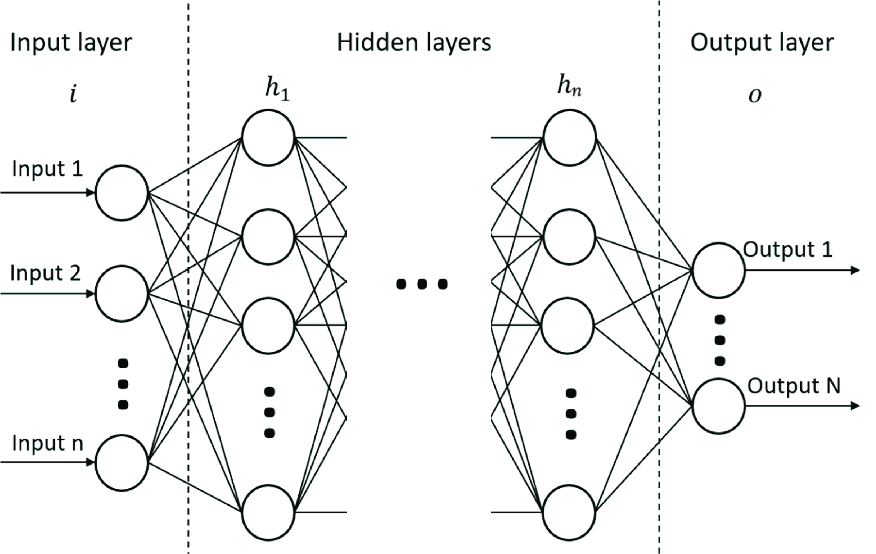
\includegraphics[width=0.8\textwidth]{images/MLP_arch.png}
	
	\caption{Architecture of multilayer perceptron \cite{MLParch}.}
	\label{fig:mlp}
\end{figure} 

\section{Recurrent neural network}
\label{theoryRNN}

In general recurrent neural network is type of neural network that in some way uses results from previous step or steps in order to improve prediction. These models are used for ordered data where next step is dependent on more than single previous one.

\subsection{Elman RNN}

Elman RNN also known as simple recurrent network (SNR) is type of recurrent neural network that utilize results of hidden layer before activation in previous step as an additional input in next one. We can see this architecture on figure \ref{fig:elman_arch}, where on left we can see how forward propagation look and on right how it looked unrolled over time, we see that middle layer which is a hidden layer of model gets two inputs, first is input vector $x_t$, where $t$ denotes step (usually time step), which is multiplied with matrix of weights $W_i$ and second one is vector $h_{t-1}$ which is result of this layer also called context vector in previous step. which is multiplied by different matrix of weight denoted as $W$, these two results after they are then summed together and result goes to activation layer which create resulting new vector $h_t$ \cite{elman}, this whole process can be summarized by this equation (where $b_i$ and $b$ are bias vectors):

\begin{equation}
	\label{eqn:elman}
	h_t = act(x_t W^T_i + b_i + h_{t-1} W^T + b).
\end{equation} 

Usually this result is directly used as output or go into single fully-connected feed-forward layer. In multi-layered version of this network, result of first hidden layer would go into next hidden layer together with result of that specific layer in previous step and again both would get multiplied by matrices of weight specific for that layer, summed and results goes through activation function.

\begin{figure}[!h]
	\centering
	
	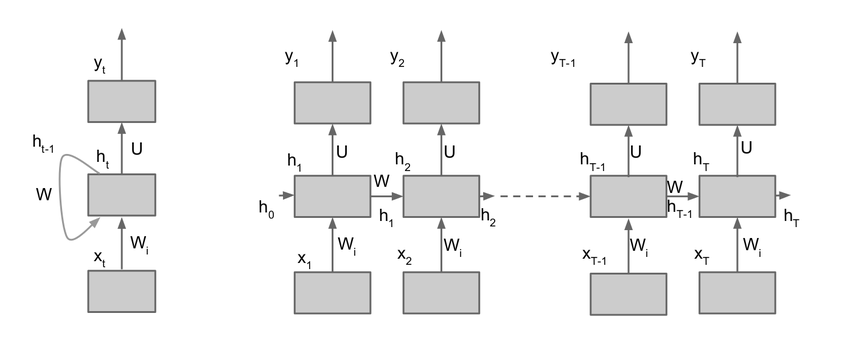
\includegraphics[width=0.85\textwidth]{images/Elman_RNN_architecture.png}
	
	\caption{Architecture of Elman RNN \cite{elman_img}.}
	\label{fig:elman_arch}
\end{figure}

\subsection{Gated Recurrent Unit}

Gated recurrent unit is more complex RNN compared to Elman RNN. This model was developed as simplification of even more complex LSTM model. We can say that it consist mainly of three parts that interact with each other and together create final prediction. Those parts are reset gate, update gate and candidate hidden state computation. We can see structure of hidden layer of GRU on figure \ref{fig:gru_arch}. On this diagram sigmoid means fully-connected feed-forward layer with sigmoid activation function and tanh means fully-connected feed-forward layer with hyperbolic tangent activation function.
\\

Reset gate is on left side of diagram, it's task is to using input and previous hidden state vectors modify previous hidden state vector which goes into candidate hidden state computation. This should helps capture short-term dependencies in time series by removing part of information from previous hidden state vector.
\\

Candidate hidden vector computation is part that is similar to Elman RNN with two differences, firstly inputted hidden layer is modified by reset gate result and secondly resulting vector from this part is only candidate which goes into further calculation. This candidate contains mostly current and short-term past information thanks to specific vectors that input consist of. 
\\

Update gate, similarly to reset gate, uses concatenation of input and previous hidden state vector on input, but this time results are used to modify both previous hidden state and candidate hidden state in a way that resulting hidden state is weighted average of those two vectors where weights are results from this gate. This should help to capture long-term dependencies in time series from previous hidden state vector and reintroducing it into final hidden state by combining it with candidate hidden state vector that should contain mostly current and short-term information. This whole architecture is shown on Fig. \ref{fig:gru_arch}.
\\

\begin{figure}[!h]
	\centering
	
	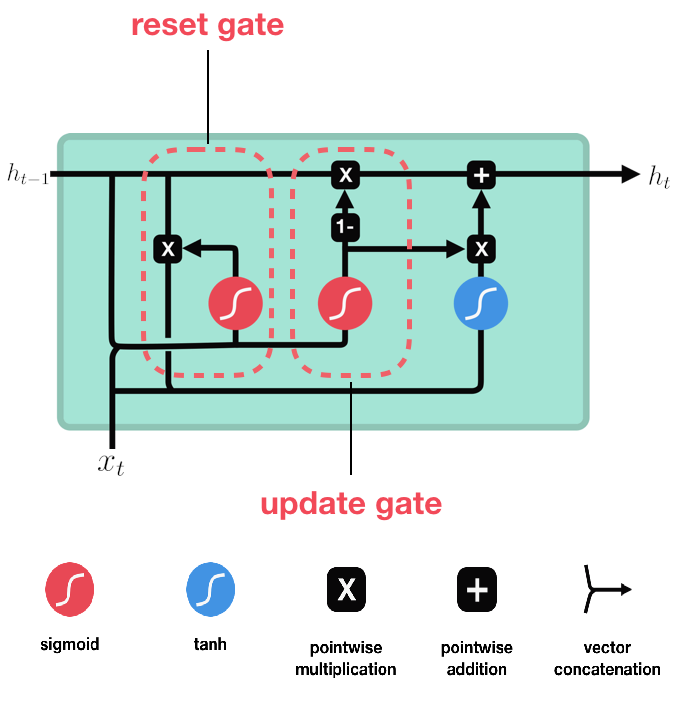
\includegraphics[width=0.6\textwidth]{images/GRU_arch.png}
	
	\caption{Architecture of GRU hidden layer.}
	\label{fig:gru_arch}
\end{figure}

Multi-layered version is achieved by stacking hidden layers where hidden state vector of one layer is input vector of next one.

\subsection{Long Short-Term Memory}

As mentioned earlier, LSTM is more complex predecessor of GRU. This model was developed with aim to mitigate vanishing gradient problem, that cause lack of long-term memory in models like Elman RNN, mainly by introducing memory vector, sometimes called memory cell, that should maintain information over longer period. As we can see in figure \ref{fig:lstm_arch} this model consist of three gates, candidate memory computation. Legend in this diagram have same meaning as one in GRU architecture diagram.
\\

All three gates and candidate memory computation has same input, which consist of input and previous hidden state vectors. In all of them this input goes into fully-connected feed-forward layer and then into activation function. In case of gates this activation function is sigmoid function, that bound all values into range (0,1), while candidate memory calculation uses hyperbolic tangent as activation function.
\\

Forget gate has the task of removing unnecessary information from memory vector by elementwise multiplication of it's result with previous memory vector. 
\\

Input gate together with candidate memory vector computation are meant to introduce new information into memory cell after adjustment from forget gate. Firstly model computes candidate memory then, then this vector is adjusted by input gate result and finally added to the modified previous memory vector. This results in new memory vector.
\\

Finally output gate is used to determine how much each part of memory should contribute into new hidden state vector. We can see diagram of this process on Fig. \ref{fig:lstm_arch}.

\begin{figure}[!h]
	\centering
	
	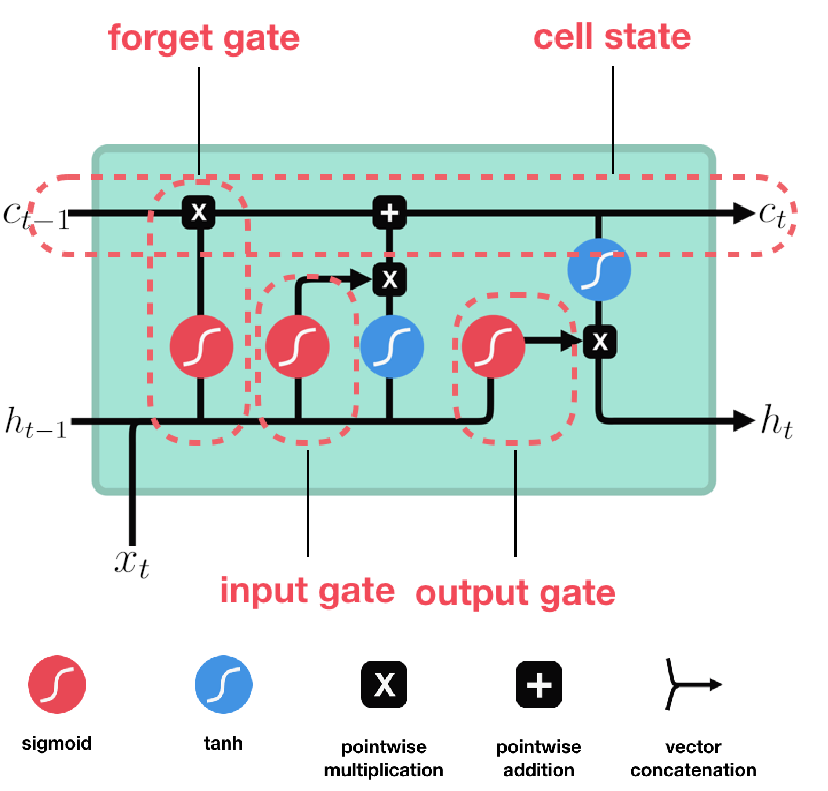
\includegraphics[width=0.6\textwidth]{images/LSTM_arch.png}
	
	\caption{Architecture of LSTM hidden layer.}
	\label{fig:lstm_arch}
\end{figure}

\section{Transformer}
\label{theoryTrans}

Transformer is a deep learning model architecture introduced in 2017 by Vaswani et al. \cite{attentionAllYouNeed} that's especially good at handling sequences, like text. This architecture consist of encoder and decoder as shown in Fig. \ref{fig:trans}. Encoder in this model is meant to contextualized representation of input while decoder takes this contextualized representation and mixes together with previous outputs to get prediction of next output. Other than these two main blocks this model usually also contains Tokenizer , Embedding layer and Positional encoding to prepare in going data and Fully-connected Feed-forward layer with softmax activation function to turn result of decoder into probability distribution of possible tokens.  

\begin{figure}[!h]
	\centering
	
	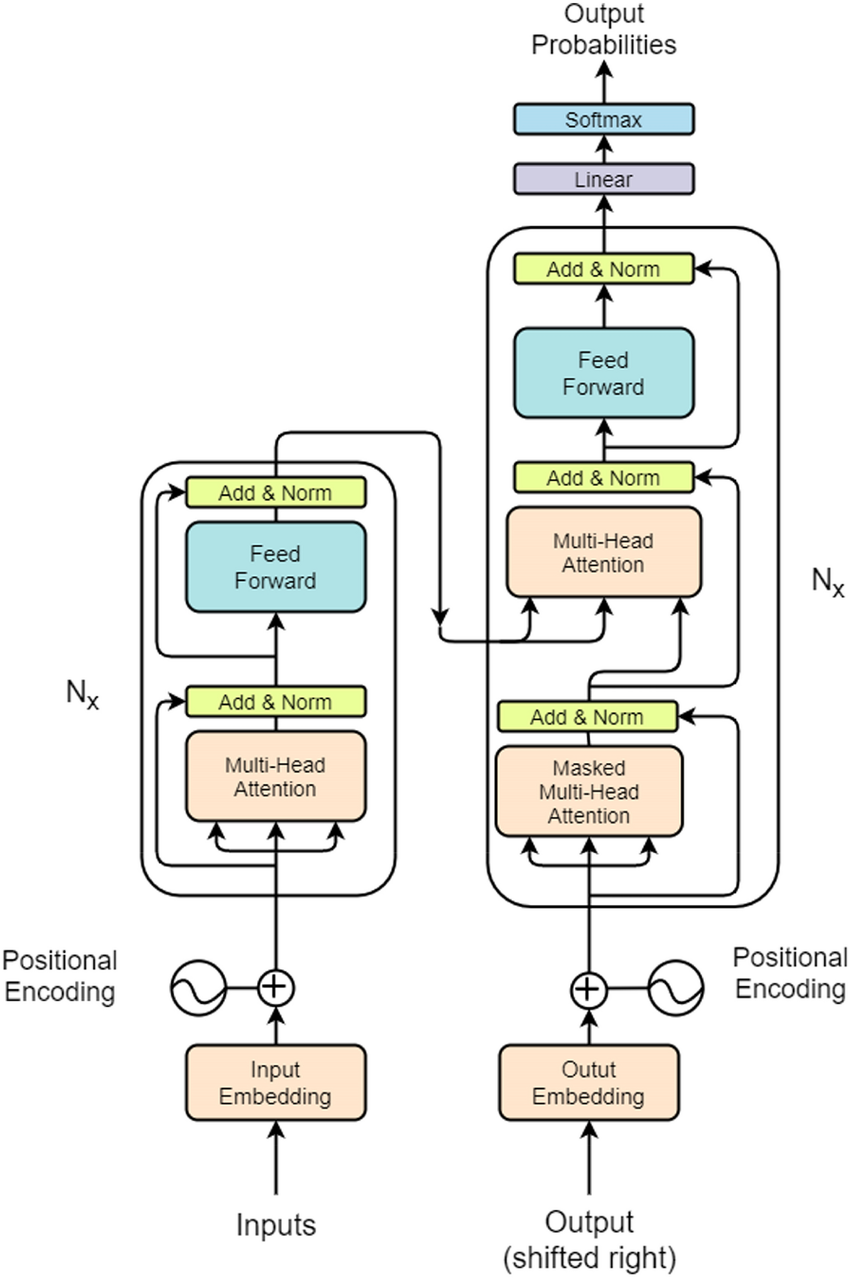
\includegraphics[width=0.6\textwidth]{images/trans_arch.png}
	
	\caption{Architecture of one encoder-decoder block in transformer model from original "Attention is all you need" paper \cite{attentionAllYouNeed}.}
	\label{fig:trans}
\end{figure}

\subsection{Tokenizer, Embedding layer and Positional encoding}

First part of Transformer model is usually input preparation, this part may differ based on type of data used. This part consist of three parts:
\\

\begin{itemize}
	\item Tokenizer - this layer split input into tokens, for example if input is textual, tokens might words or syllables
	\item Embedding layer - task of this layer is to transform each one of input tokens into numerical vectors of same length
	\item Positional encoding - finally last preparation layer add to each embedding of token vector which encodes their position with regards to other tokens
\end{itemize}

In most cases Tokenizer and Embedding layer are trained separately and do not change during training if Transformer while Positional encoding is trained alongside rest of Transformer.

\subsection{Encoder}
\label{theoryEncoder}

Encoder architecture consist of multiple attention blocks where each block consist of multi-headed Self-attention and Multi-layered Feed-forward Neural Network, after each of these step embeddings from step input are added to output and result is layer normalized, adding of step input embedding is done to create residual paths that helps mostly with vanishing gradient problem and layer normalization then helps by making sure results neither explode neither go to zero as well as it bring bit of additional non-linearity to model. Firstly input embeddings are split into parts that each goes into separate head  Self-attention.
\\

Architecture of Self-attention is shown on Fig. \ref{fig:self_att} where we can see that each input token get multiplied by key, query and value matrices to receive their key, query and value vectors, after that each query is multiplied with each key to create attention matrix which should encode how much each token influence other, after that matrix goes into column wise softmax function to normalize it and finally it's multiplied my matrix of value vectors to create new embedding of tokens that should contain not only original information but also influence information. 
\\

\begin{figure}[!h]
	\centering
	
	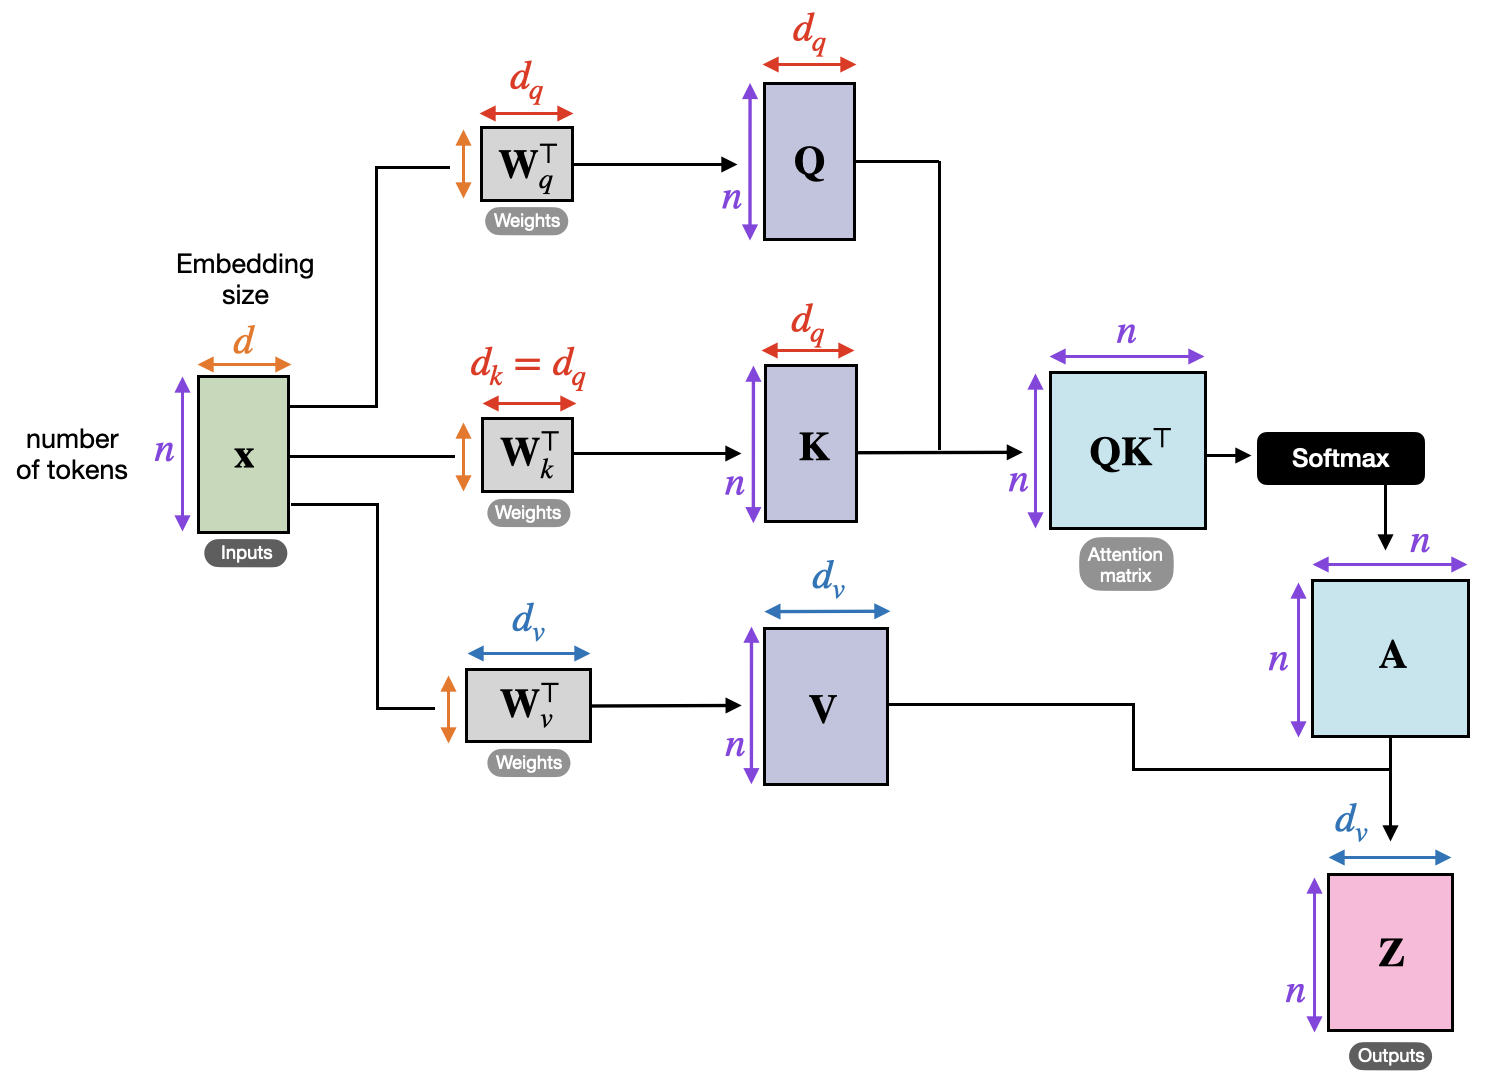
\includegraphics[width=1\textwidth]{images/self_attention.png}
	
	\caption{Architecture of Self-attention mechanism.}
	\label{fig:self_att}
\end{figure}

Results of each Self-attention head are then concatenated back into new embeddings that have same dimensions as original ones, then after adding residual connection and normalization results goes into Multi-layered Feed-forward Neural Network to further extract information from embeddings.

\subsection{Decoder}

Architecture of decoder, similarly to encoder, consist of multiple attention blocks, however in this case attention block consist of three parts instead of two. 
\\

First is masked multi-headed Self-attention which is similar to unmasked Self-attention with only difference being application of masking to the attention matrix before softmax function to make sure that words on some specific positions does not affect words on other specific positions. Decoder use what's called casual or look-ahead masking which forbid future tokens to affect past ones, in our case this guarantees that record cannot be affected by record which happened after so in the future from it's perspective. 
\\

Second part is multi-headed Cross-attention, which takes two lists of token embeddings and compute effect of tokens in first list onto tokens in second list. In this case key and value vectors are computed from contextualized representation computed by encoder while query vectors are computed from results of self-attention in decoder, other than that remaining architecture is same as unmasked Self-attention. 
\\

Final part of decoder attention block is multi-layered feed-forward neural network that further extract information from embeddings. 

\subsection{Fully-connected Feed-forward layer}

After that results of decoder goes into final Fully-connected Feed-forward layer which change dimensionality of the decoder output from embedding size into vocabulary and apply softmax activation on result. This way we expect to get in last token probability distribution through all possible tokens. In our case we changed this last part. We run into problem where most of our records (our tokens) are unique creating extremely large vocabulary, this was caused partially by many possible combinations of disease, drug and medical procedure which are encoded in record and partially by timestamp which add additional uniqueness since it's improbable that two patients would get for example same drug, for same disease, at same age. Because of this we decided to remove softmax activation, changing fully-connected feed-forward layer in a way that result maintain dimension of embedding and added function that split result, find closest embedding of each part and concatenate result together leaving us with specific new embedding prediction instead of probability distribution.

\subsection{Decoder-only Transformer}

Decoder-only version of Transformer model is simplified version of model which completely exclude Encoder part of model and from Decoder part it excludes Cross-attention mechanism. This model is usually used if we wanna generate next tokens without having stable context that would normally go into Encoder part.
\\

This means that this simplified architecture is much more similar to standard RNN in terms of input and expected output.

\section{Language-agnostic BERT Sentence Embedding}
\label{theoryLaBSE}

Language-agnostic BERT Sentence Embedding model also known under abbreviation LaBSE is model trained with main goal being to generate similar representation to pairs of sentences which have same meaning and are only translations in two different language \cite{labse_kaggle}. 
\\

Architecture of LaBSE model consist of 4 parts \cite{labse_hug}:

\begin{enumerate}
	\item Encoder-only transformer (BERT model)
	\item Pooling layer
	\item Dense layer
	\item Normalization layer
\end{enumerate}

\subsection{Encoder-only Transformer (BERT model)}
\label{emb:trans}

First and most important part of LaBSE model is transformer, which is a deep learning architecture. More specifically LaBSE uses BERT so bidirectional encoder representations from transformers model which is encoder-only transformer architecture meaning this model does not contain decoder found in standard transformer which is usually used for prediction, because of this BERT model is focused in extracting contextual information from input text. Architecture of standard BERT model looks like this: 

\begin{enumerate}
	\item Tokenizer layer
	\item Embedding layer
	\item Encoder
	\item Task layer
\end{enumerate}

\subsubsection{Tokenizer layer}

First layer is tokenizer, this layer takes input text split it into tokens which in case of BERT model is called PieceWise tokenizer which split text into subwords so something close to syllables. PieceWise tokenizer has advantage compared to different tokenizers that use either words or characters. Compared to character wise tokenizing, subwords contain more information than characters, and compared to word tokenizer is that there a lot less subwords than words and are more similar across multiple languages, creating much smaller vocabulary which is especially important for multilingual models. After split this layer assign integer number to each unique token, LaBSE model vocabulary distinguishes around 500 000 different tokens.

\subsubsection{Embedding layer}

After that comes embedding layer which assign real number vector to each token, more specifically BERT model compute three different embeddings and add them together and normalize result to get final one. First is token type embedding, which is basic embedding where each token in vocabulary is assigned it's unique embedding. Second is positional embedding, as name suggest this embedding contain information about where in the sequence token is found giving additional information. Third and final embedding is segment type, which encodes information about to which segment, usually sentence token belong, important for embedding input text consisting of multiple sentences.

\subsubsection{Encoder}

Third and most important layer is encoding. This is the layer in which contextual information are mined from the text. Architecture of this layer is same as architecture explained in Sec. \ref{theoryEncoder}. In case of BERT used in LaBSE there are 12 attention blocks. 

\subsubsection{Task layer}

Each head of self-attention layer takes a input set of embeddings and to compute new set of embeddings which should encode not only original information but also information about relationship between original ones, in other words it encodes effect of tokens onto each other. To do that it compute for each input embedding three vectors usually called key, query and value by multiplying input embedding with three matrices which values are learned during training. After that to get new embedding query vector is multiplied with matrix created from key vectors so resulting vector is vector of dot product of single query and all keys, this vector then goes through softmax function to normalize result. In some transformer models before softmax this vector get masked. Masking is done by setting values where key vector belongs to later embedding than query to minus infinity, this way after softmax this values become zeros. This is done so that later embedding does not affect previous ones. It's mostly useful in models trained to predict next token in order for model to learn to predict only based on tokens from past on not future. However in case of model like BERT where emphasis is on extracting as much information from input text masking is not done. Final step to get new embedding is to multiply vector we got after applying softmax with matrix composed of value vector to get linear combination of value vectors. This resulting vector is new embedding. This is done for all query vectors. List list resulting vectors is output embedding of attention head. Since this model use multi-headed attention more specifically in case of LaBSE 12-headed attention, this process is simultaneously independently done 12 times and results of each head are than concatenated into final result of attention. By using multiple head we expect that each head can extract different information from input and final concatenation give us result that contains all extracted information.    
\\

This concatenation of new embeddings goes than into multi-layered feed-forward neural network sometimes also called Multilayer Perceptron or MLP for short, architecture of this model is explained in Sec. \ref{MLP}.
\\

Result goes to next attention block and process is repeated again. Result of final attention block then goes to last part which is task layer, this layer can be viewed as simple decoder that map resulting embeddings back into token space. Based on this results is then model pre-trained. Training process of BERT model usually consist of two tasks on which are model trained at the same time. First is Masked Language Modeling (MLM) where 15\% of input tokens are masked meaning either replaced by mask placeholder or by random different token, after that masked input goes into model, then from resulting tokens are taken those on position of masked tokens in input and are compared to correct token before masking which creates error that is back-propagated through model updating it's parameters \cite{bert_pretr_1}. Other task usually used is called Next Sentence Prediction (NSP), in this task model gets input which start with special classify token and after that two spans of texts separated by special separator token. Task of model is to say whether these two spans of text can appear one after another or more precisely whether they appeared one after another in training corpus and put this information into first token of result encoded by two special tokens either "is next" or "not next" token and similarly difference between expected and resulting first token create error that back-propagates through model \cite{bert_pretr_2}. However in some BERT-based model like LaBSE second task is replaced with translation language modeling (TLM), this task is extention of MLM in which model gets two concatenated sentence instead of one and where the second sentence is translation of the first in another language, rest of the task is than same as in MLM, so whole input gets masked and model is tasked to predict masked tokens \cite{bert_pretr_3}. Task layer is used primarly in only during pre-training and is omitted when model is used for different task as many use-cases does not need tokens in results but use embeddings from encoding layer as form of text encoding which is that further used in task specific layers on which then model is fine-tuned.

\subsection{Pooling layer}

After BERT model returns embeddings of all input tokes, these then needs to be aggregated into single vector which corresponds to embedding of whole input. This aggregation is done using pooling layer. In case of LaBSE this pooling is done simply by taking embedding of first token which is an embedding of special classify token added to beginning of BERT input.    

\subsection{Dense layer}

Next layer is standard feed forward dense layer with use hyperbolic tangent activation function. Number of input and output neurons is same, and additional bias neuron is used.

\subsection{Normalization layer}

Final layer is normalization which task is only to normalize resulting vector, so divide vector by number in order to have final vector with $L_2$ norm equal one.

\section{Word2vec model}
\label{theoryW2v}

Word2vec is a neural network-based method for generating word embeddings, which are dense vector representations of words that capture their semantic meaning and relationships, in other words properties like distance between two embeddings contains some underlying information about those words such as their similarity. There are two main approaches to implementing Word2vec:

\begin{itemize}
	\item Continuous bag-of-words (CBOW) 
	\item Skip-gram
\end{itemize}

\subsection{CBOW approach}

Model using CBOW approach gets sequence of words called context with one being missing and on the output it's trying to predict missing target word. Model initially assign one-hot encoding to each word in it's dictionary. During training, each word from context is firstly converted into it's one hot encoded embedding which is then multiplied by weight matrix to get their lower dimensional dense embedding, dense embedding of all words in context are then averaged out and resulting embedding goes into hidden layer which transform vector back into dimension of vocabulary, finally softmax function is applied to get probability of each word from vocabulary to be predicted as missing word. We can see this architecture in \ref{fig:cbow_arch}. Training is usually done using fixed context window moving along training text.

\begin{figure}[!h]
	\centering
	
	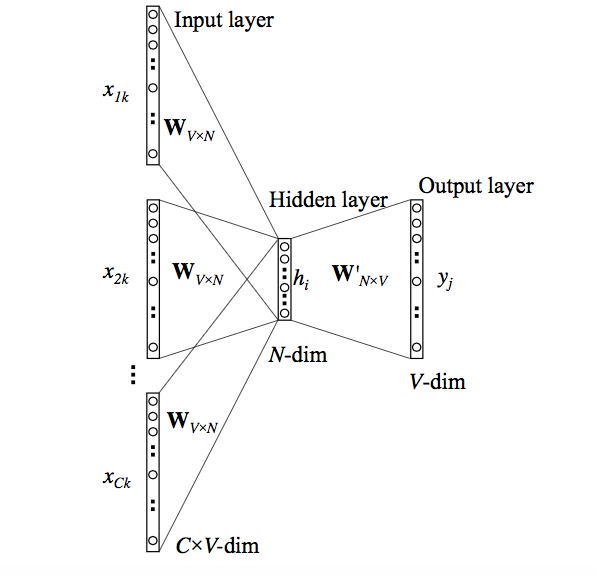
\includegraphics[width=1\textwidth]{images/CBOW_arch.png}
	
	\caption{Architecture of NN to train CBOW implenetation of Word2vec model \cite{cbow}.}
	\label{fig:cbow_arch}
\end{figure}

\subsection{Skip-gram approach}

Skip-gram approach works in opposite way, where model gets target word and is trying to predict context around it. Similarly to CBOW, input word is firstly one-hot encoded then multiplied by weight matrix to transform it into dense encoding, the goes into next layer to transform it back into dimension of vocabulary goes into softmax creating vector of probabilities of surrounding context words. Error of Skip-gram is the sum of the negative log-likelihood of all context words. We can see this architecture in \ref{fig:skip_arch}.

\begin{figure}[!h]
	\centering
	
	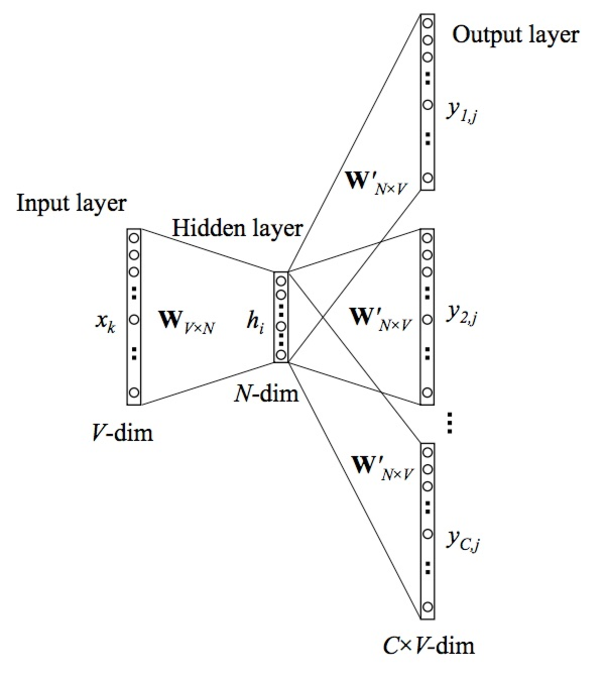
\includegraphics[width=1\textwidth]{images/Skip_arch.png}
	
	\caption{Architecture of NN to train Skip-gram implenetation of Word2vec model \cite{skipgram}}
	\label{fig:skip_arch}
\end{figure}
\\ 